\chapter{Operational definition: 은유가 아니라 causal boundary}
\label{STC-S02}

\section{엄격한 정의}

본 연구에서 \stc{}는 다음 다섯 조건을 모두 만족하는 computation이다.

\begin{enumerate}
  \item \textbf{Wake-derived input}: 실제 interaction, feedback, tool trace, retrieved memory, model
        failure 또는 그에 연결된 evidence를 입력으로 삼는다.
  \item \textbf{Deferred causal boundary}: 현재 response의 latency-critical dependency가 끝난 뒤
        실행되며 현재 답을 완성하기 위한 필수 compute가 아니다.
  \item \textbf{Reusable destination}: 후속 session/query가 읽을 persistent 또는 bounded-lifetime
        state를 바꾼다.
  \item \textbf{Transformation}: append만 하지 않고 select, summarize, link, replay, train, edit,
        distill, compress, merge, evict 중 하나 이상을 수행한다.
  \item \textbf{Validation/publication}: 후보 state와 serving state의 경계를 두고 실패 시 reject 또는
        rollback할 수 있다.
\end{enumerate}

즉 sleep-time compute는 latency-critical response 뒤로 연기되고, 다음 wake episode가 재사용할
state를 바꾸는 lifecycle이다.\claim{STC-C005} 이 정의는 Model Needs Sleep의 post-response consolidation,
OpenAI Dreaming의 background synthesis, Mem0 Dream의 scheduled transformation에 공통으로 적용된다
\parencite{srcstc0014,srcstc0052,srcstc0063}.

\begin{figure}[htbp]
  \centering
  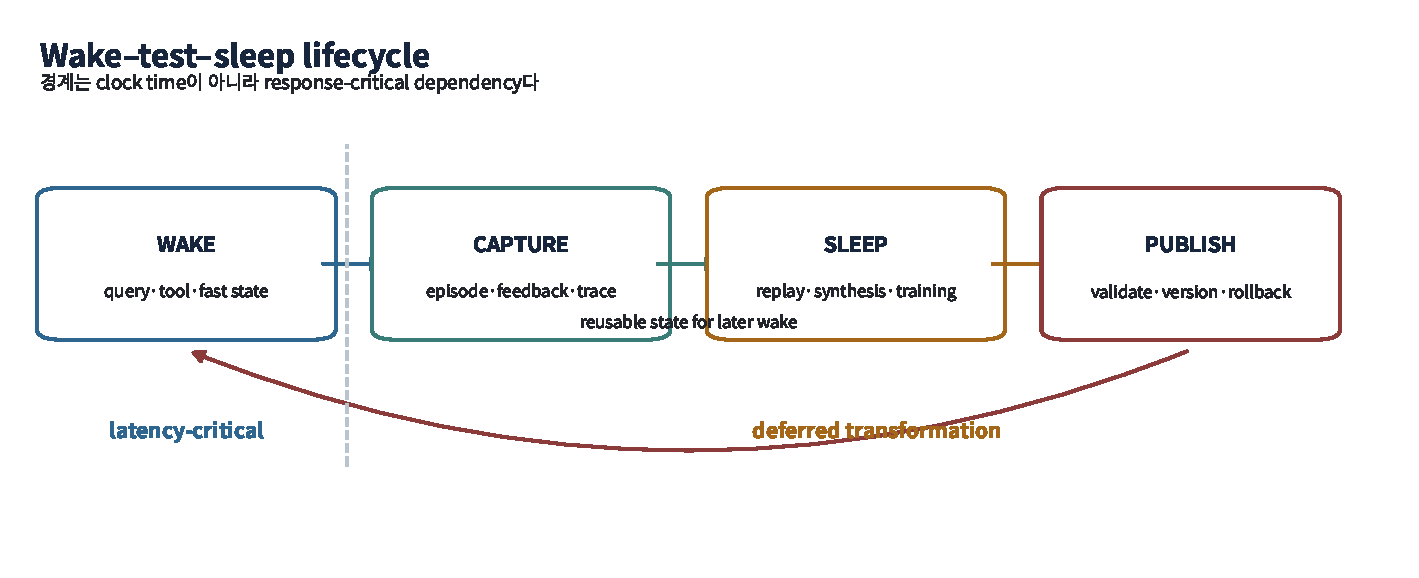
\includegraphics[width=0.98\textwidth]{figures/stc-f001.pdf}
  \caption{Wake--capture--sleep--publication의 causal lifecycle. 점선 경계 왼쪽은 현재 response의
  latency-critical path이고, 오른쪽은 후속 wake용 state를 만드는 deferred path다.}
  \stcfigure{STC-F001}
  \figsource{Original synthesis; SRC-STC-0014, SRC-STC-0052}{Wake, capture, sleep, publish 네 상자가 순서대로 연결되고 검증된 재사용 상태가 다음 wake로 되돌아오는 순환도.}
  \label{fig:stc-lifecycle}
\end{figure}

\section{Timing과 medium은 직교한다}

Update timing과 memory medium은 독립 축이다. Sleep phase는 weights, adapters, recurrent state,
text/vector store, temporal graph 또는 mixture를 바꿀 수 있다.\claim{STC-C006} 따라서 ``weights를
바꾸지 않으면 training이 아니므로 sleep도 아니다''와 ``background에서 실행되면 모두 sleep이다''는
둘 다 너무 좁거나 넓다.

\begin{figure}[htbp]
  \centering
  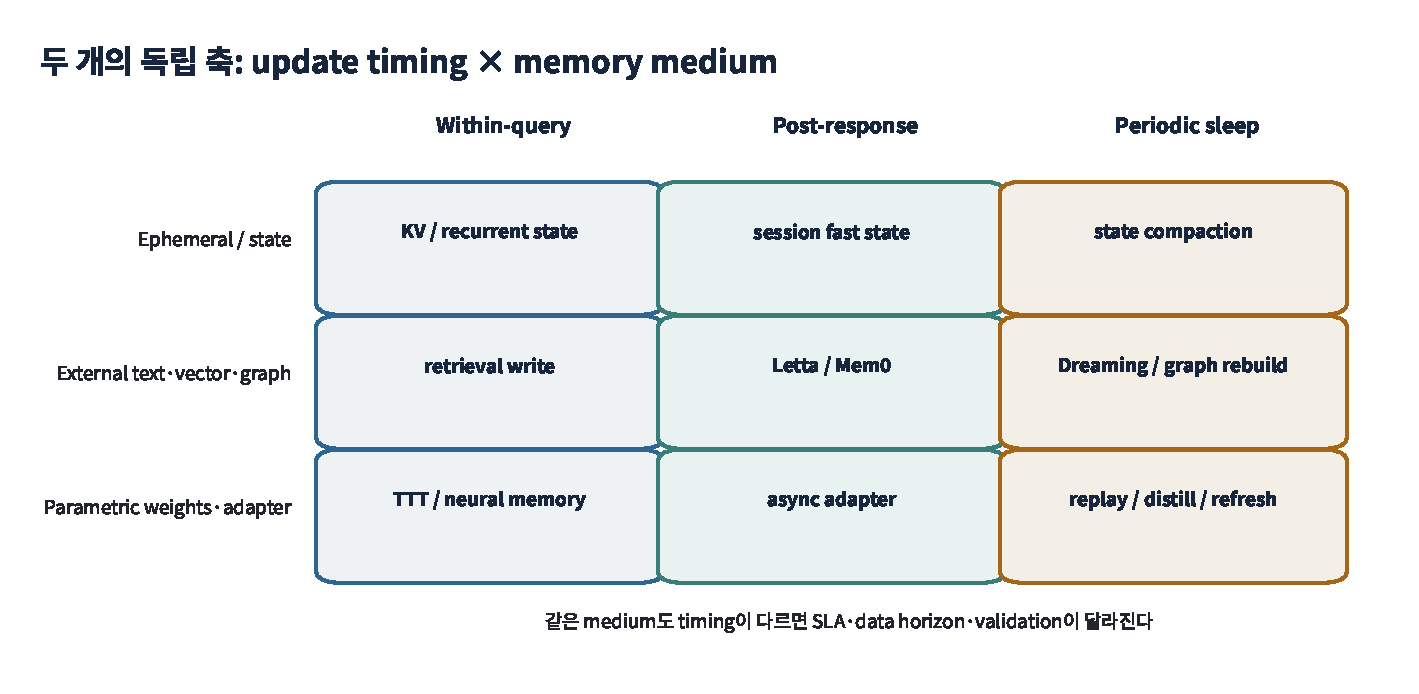
\includegraphics[width=0.98\textwidth]{figures/stc-f002.pdf}
  \caption{Update timing과 memory medium의 3$\times$3 taxonomy. 같은 LoRA update도 current answer 전에
  수행하면 test-time training, response 뒤에 수행하면 asynchronous consolidation이다.}
  \stcfigure{STC-F002}
  \figsource{Original synthesis; SRC-STC-0014, SRC-STC-0021, SRC-STC-0016}{열은 query 내부, response 이후, 주기적 sleep이고 행은 ephemeral state, 외부 text-vector-graph, parametric weight-adapter인 격자.}
  \label{fig:stc-taxonomy}
\end{figure}

분류를 위해 각 operator를 6-tuple로 기록한다.

\begin{equation}
O=(t_{trigger}, D_{horizon}, M_{source}, M_{dest}, S_{scope}, P_{publish}),
\end{equation}

여기서 trigger는 언제 시작하는지, $D_{horizon}$은 어느 기간 data를 보는지, source/destination medium은
무엇인지, scope는 query/session/user/cohort/global 중 어디인지, publication policy는 어떻게 후보를
활성화하는지 나타낸다. 같은 architecture라도 이 tuple이 다르면 system workload가 다르다.

\section{포함과 제외}

\begin{table}[htbp]
\centering
\caption{본 연구의 포함·제외 판정}
\label{tab:stc-inclusion}
\small
\begin{tabularx}{\textwidth}{p{0.27\textwidth} X X}
\toprule
행동 & 판정 & 이유 \\
\midrule
현재 query의 long chain-of-thought & 제외 & persistent reusable state를 바꾸지 않음 \\
token-by-token TTT 후 현재 답 생성 & wake/test-time & 현재 response dependency 안에 있음 \\
post-response memory agent가 profile 수정 & 포함 & deferred transformation + later reuse \\
nightly vector re-embedding/index rebuild & 포함 & external reusable state 변환 \\
LRU가 cache line을 passive eviction & 제외 & learned/validated consolidation이 아님 \\
주기적 global continued pre-training & 조건부 포함 & wake-derived stream과 explicit later-use lifecycle이면 포함 \\
배포 전 generic offline training & 제외 & wake experience와 persistent deployed loop가 없음 \\
검증 없는 background summary append & 미완성 & transformation은 있지만 publication/gate가 부재 \\
\bottomrule
\end{tabularx}
\end{table}

\section{Sleep phase와 biological stages}

NREM/REM은 replay와 perturbation, integration과 abstraction을 생각하게 하는 productive analogy다.
그러나 구현은 EEG stage를 모방할 필요가 없다. 본 연구는 기능을 다음처럼 매핑한다.

\begin{itemize}
  \item NREM-like: high-fidelity replay, recent episode integration, stable fact linking,
  \item REM-like: perturbed/generative replay, abstraction, counterfactual strategy discovery,
  \item publication: biological analogy에는 약하지만 production system에는 필수인 validation·rollback.
\end{itemize}

마지막 항이 중요한 이유는 agent memory가 사용자 data와 serving artifact를 다루기 때문이다. Biology는
배울 mechanism을 제공하지만 tenant scope, deletion SLA, source license, atomic rollout을 해결하지 않는다.

\begin{cautionbox}[Phase와 mechanism을 혼동하지 말 것]
Sleep은 \emph{언제와 어떤 lifecycle에서} 변환하는지, replay·distillation·RL·editing은 \emph{어떻게}
변환하는지, weights/text/vector/graph는 \emph{어디에} 저장하는지를 답한다. 세 질문을 분리해야
동일 resource에서 matched baseline을 만들 수 있다.
\end{cautionbox}
